\documentclass[12pt,titlepage]{article}
\usepackage[margin=1.25in]{geometry}
\usepackage{graphicx,amsmath,minted}

%% Variables definition
\newcommand{\vSubject}{Object Oriented Programming}
\newcommand{\vSubtitle}{Midterm Exam}
\newcommand{\vName}{Dicha Zelianivan Arkana}
\newcommand{\vNIM}{2241720002}
\newcommand{\vClass}{2i}
\newcommand{\vDepartment}{Information Technology}
\newcommand{\vStudyProgram}{D4 Informatics Engineering}

%% [START] Tikz related stuff
\usepackage{tikz}
\usetikzlibrary{svg.path,calc,shapes.geometric,shapes.misc}
\tikzstyle{terminator} = [rectangle, draw, text centered, rounded corners = 1em, minimum height=2em]
\tikzstyle{preparation} = [chamfered rectangle, chamfered rectangle sep=0.75em, draw, text centered, minimum height = 2em]
\tikzstyle{process} = [rectangle, draw, text centered, minimum height=2em]
\tikzstyle{decision} = [diamond, aspect=2, draw, text centered, minimum height=2em]
\tikzstyle{data}=[trapezium, draw, text centered, trapezium left angle=60, trapezium right angle=120, minimum height=2em]
\tikzstyle{connector} = [line width=0.25mm,->]
%% [END] Tikz related stuff

%% [START] Fancy header related stuff
\usepackage{fancyhdr}
\pagestyle{fancy}
\setlength{\headheight}{15pt} % compensate fancyhdr style
\fancyhead{}
\fancyfoot{}
\fancyfoot[L]{\thepage}
\fancyfoot[R]{\textit{\vSubject - \vSubtitle}}
\renewcommand{\footrulewidth}{0.4pt}% default is 0pt, overline for footer
%% [END] Fancy header related stuff

%% [START] Custom tabular command related stuff
\usepackage{tabularx}
\newcommand{\details}[2]{
    #1 & #2  \\
}
%% [END] Custom tabular command related stuff

%% [START] Figure related stuff
\newcommand{\image}[3][1]{
    \begin{figure}[h]
        \centering
        \includegraphics[#1]{#2}
        \caption{#3}
        \label{#3}
    \end{figure}
}
%% [END] Figure related stuff

\begin{document}
\begin{titlepage}
    \centering
    \vfill
    {\bfseries\LARGE
        \vSubject\\
        \vskip0.25cm
        \vSubtitle
    }
    \vfill
    
\includegraphics[width=6cm]{images/polinema-logo.png}
    \vfill
    {
        \textbf{Name}\\
        \vName\\
        \vskip0.5cm
        \textbf{NIM}\\
        \vNIM\\
        \vskip0.5cm
        \textbf{Class}\\
        \vClass\\
        \vskip0.5cm
        \textbf{Department}\\
        \vDepartment\\
        \vskip0.5cm
        \textbf{Study Program}\\
        \vStudyProgram
    }
\end{titlepage}

\section{How to write a class}
Based on the code below, please explain if the code is correct or not.

\begin{minted}[autogobble,fontsize=\small]{java}
    public class ClassA {
        float fl = 0.15f;

        float hitung() {
            float x = 2f * f1;
        }
    }
\end{minted}

The code above is still \textit{incorrect} because the \texttt{hitung()} method does not return any value. The correct code should be like this:

\begin{minted}[autogobble,fontsize=\small]{java}
    public class ClassA {
        float fl = 0.15f;

        float hitung() {
            float x = 2f * f1;
            return x;
        }
    }
\end{minted}

\section{Sum of 2 dimensional array}
Write a java code to calculate the sum of a 2 dimensional array using a loop.

\begin{minted}[autogobble,fontsize=\small]{java}
    public class SoalArray {
        public static void main(String[] args) {
            int[][] arrayInt = {
                {1, 1, 4},
                {2, 1, 2},
                {3, 2, 1}
            };

            int sum = 0;
            for (int i = 0; i < arrayInt.length; i++) {
                for (int j = 0; j < arrayInt[i].length; j++) {
                    sum += arrayInt[i][j];
                }
            }

            System.out.println(sum);
        }
    }
\end{minted}

\pagebreak

\section{Attribute and Methods inheritance}
Mention what attributes and methods that has been inherited by the class \texttt{ClassY} from the class \texttt{Class}.
Also explain how the code works!

\begin{minted}[autogobble,fontsize=\small]{java}
    public class Class {
        int a = 2;
        int x = 0;

        int hitung() {
            x = x + 5 * a;
            return x;
        }
    }

    public class ClassY extends Class {
        int b = 5;
        int y = 0;

        int hitungY() {
            y = hitung() * b;
            return y;
        }

        public static void main(String[] args) {
            ClassY cy = new ClassY();
            System.out.println(cy.hitungY());
        }
    }
\end{minted}

The attributes and methods that has been inherited by the class \texttt{ClassY} from the class \texttt{Class} are \texttt{a}, \texttt{x}, and \texttt{hitung()}.
The \texttt{hitungY} method works by calling the \texttt{hitung()} method from the parent class, then multiply the result with the \texttt{b} attribute.

\section{Class with constructor}
Inside the class below, complete the code with:
\begin{enumerate}
    \item {
        Add constructor to fill the \texttt{nim}, \texttt{name}, \texttt{address} and \texttt{gender}.
    }
    \item {
        Instantiate the object and fill the attributes through the constructor.
    }
\end{enumerate}

\pagebreak

\begin{minted}[autogobble,fontsize=\small]{java}
    public class Student {
        String nim, name, address;
        char gender;

        public Student(String nim, String name, String address, char gender) {
            this.nim = nim;
            this.name = name;
            this.address = address;
            this.gender = gender;
        }

        public static void main(String[] args) {
            Student s = new Student(
                "2241720002",
                "Dicha Zelianivan Arkana",
                "Jl. Terusan Kembang Turi",
                'M'
            );
        }
    }
\end{minted}

\pagebreak

\section{OOP}
Translate the class diagram below into a working code using OOP!

\begin{center}
    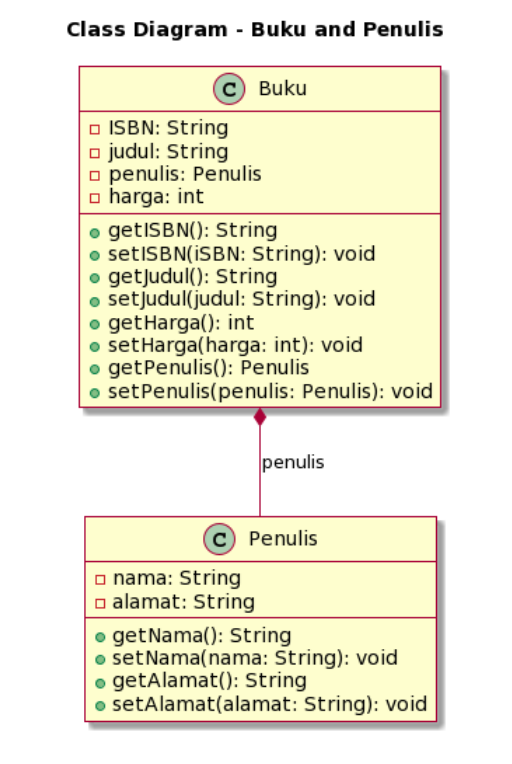
\includegraphics[height=10cm]{./images/class-diagram.png}
\end{center}

\begin{minted}[autogobble,fontsize=\small]{java}
    public class Buku {
        private String isbn;
        private String title;
        private Writer writer;
        private int price;

        public getIsbn() {
            return isbn;
        }

        public setIsbn(String isbn) {
            this.isbn = isbn;
        }

        public getTitle() {
            return title;
        }

        public setTitle(String title) {
            this.title = title;
        }

        public getWriter() {
            return writer;
        }

        public setWriter(Writer writer) {
            this.writer = writer;
        }

        public getPrice() {
            return price;
        }

        public setPrice(int price) {
            this.price = price;
        }
    }

    public class Writer {
        private String name;
        private String address;

        public getName() {
            return name;
        }

        public setName(String name) {
            this.name = name;
        }

        public getAddress() {
            return address;
        }

        public setAddress(String address) {
            this.address = address;
        }
    }
\end{minted}

\end{document}
